% Provenance (never printed): old premiere S / seconde material on minerals and
% rocks (identifying minerals in hand specimen, the silicates, the minerals of
% granite, basalt and peridotite, thin sections in polarised light).
% Element fractions and rock densities from figdata/grade-11/mineral_density.py
% (Rudnick and Gao 2014 bulk crust; webmineral mean densities). Mineral, crystal,
% rock families and the Mohs scale are Book 1's (grade 6): recalled, not defined.
% Felsic and mafic belong to g11.08: not used here.
\chapter{Mineral}\label{ch:g11:minerals}

Ambillah sebutir kerikil granit dan amatilah dengan kaca pembesar. Kerikil itu
bukan satu zat, melainkan mozaik butir-butir yang saling mengunci: butir kelabu,
seperti kaca dan hampir bening; butir merah muda, berbentuk balok, yang
permukaan patahnya berkilat terkena cahaya ketika kerikil itu diputar; serpih
hitam kecil yang dapat dicungkil ujung pisau menjadi lembaran tipis. Setiap jenis
butir adalah sebuah mineral. Bab ini menunjukkan bagaimana ahli geologi
membedakannya, mengapa hampir semuanya tersusun dari silikon dan oksigen,
bagaimana mineral-mineral itu membentuk batuan yang telah kita jumpai sejauh ini
--- granit, basalt, \omterm{def:g11:ocean-ridges:peridotite}{peridotit} --- dan bagaimana irisan batuan yang lebih tipis
daripada sehelai rambut, bila dilihat dalam cahaya terpolarisasi, memperlihatkan
semuanya sekaligus.

\begin{omfigure}
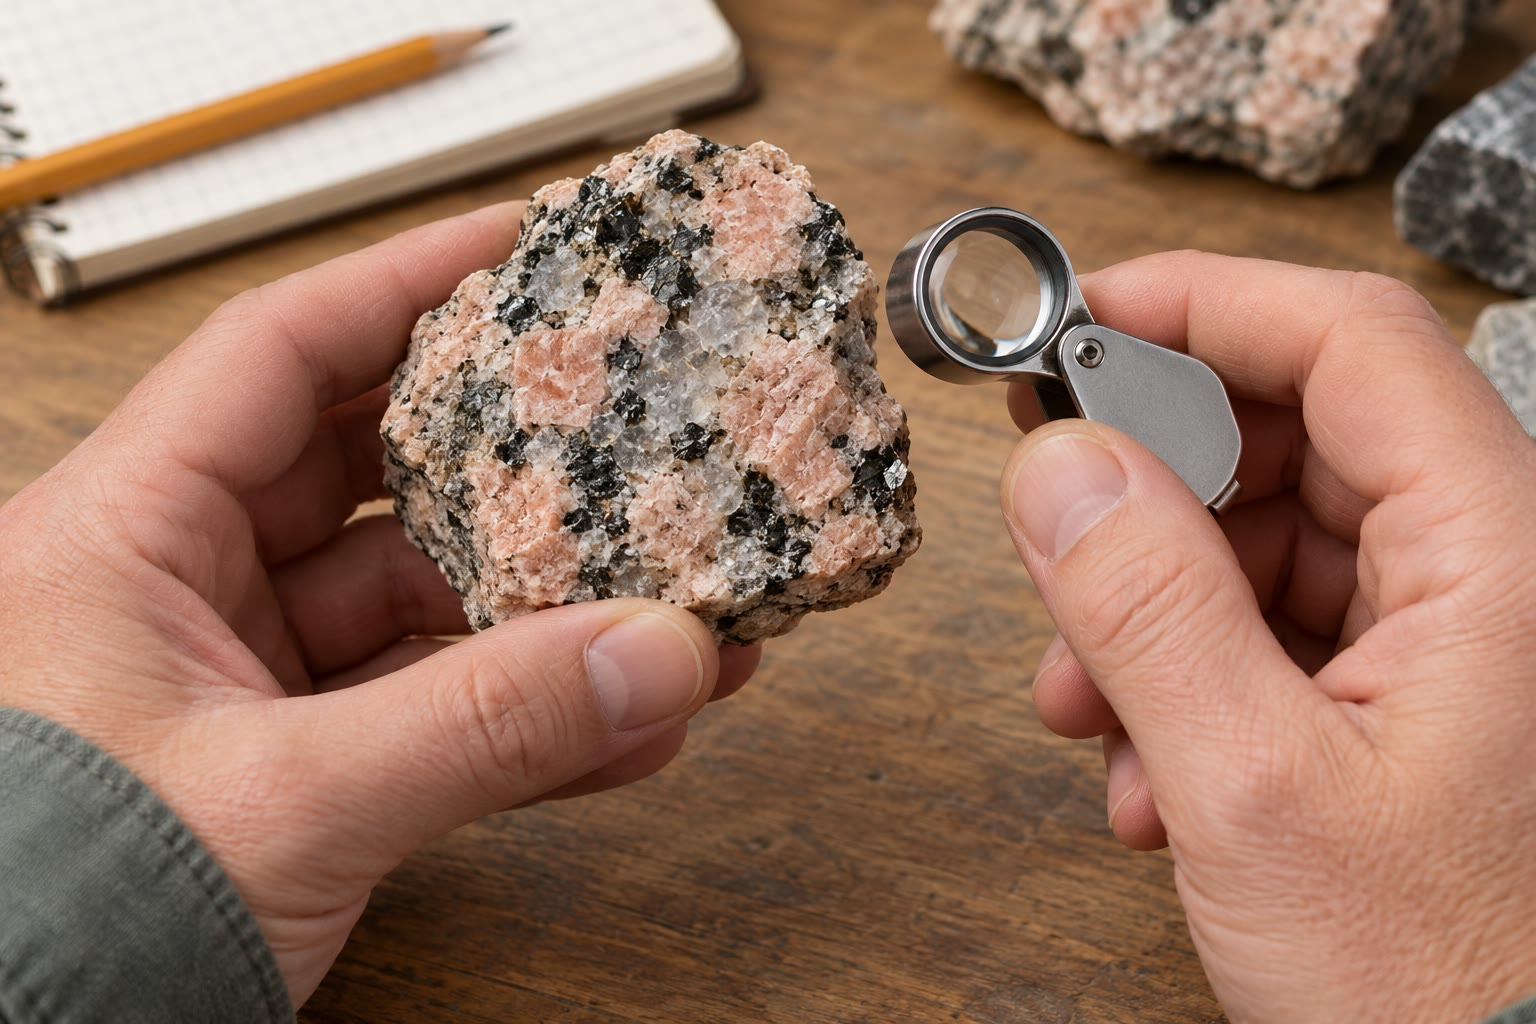
\includegraphics[width=0.62\linewidth]{images/book2/ai/g11-geologist-hand-lens.jpg}

{\small Granit yang diamati dengan kaca pembesar: alat pertama untuk membedakan
mineral-mineral. (Ilustrasi AI.)}
\end{omfigure}

\begin{recall}
Mineral adalah zat padat alami, yang tidak dibuat oleh makhluk hidup, dengan
susunan yang tetap dan atom-atom yang tertata secara teratur; batuan terdiri atas
satu atau beberapa mineral. Granit sebagian besar terdiri atas feldspar, kuarsa,
dan mika. Batuan terbagi menjadi tiga golongan, batuan beku, sedimen, dan
metamorf. Kekerasan sebuah mineral adalah seberapa baik mineral itu menahan
goresan, yang diurutkan dari 1 (talk) sampai 10 (intan) pada skala Mohs;
feldspar ortoklas berkekerasan 6 dan kuarsa 7, sedangkan pelat kaca sekitar 5.5
dan paku baja sekitar 6.5 (Buku 1, kelas 6). Massa jenis sebuah benda adalah
massanya dibagi volumenya (fisika). Senyawa diperikan oleh rumus yang menghitung
atom-atomnya; dalam zat padat yang tersusun dari ion, muatan positif dan negatif
seimbang (kimia). \omterm{def:g11:ocean-ridges:peridotite}{Peridotit} membentuk mantel; \omterm{def:g11:ocean-ridges:gabbro}{gabro} dan basalt membentuk \omterm{def:g11:ocean-ridges:oceanic-lithosphere}{kerak
samudra} (\cref{ch:g11:ocean-ridges}).
\end{recall}
% ledger: usgs:mineral-rock, nps:granite-minerals, nps:mohs-ladder, nps:mohs-testers

\section{Membedakan mineral}

Mineral mempunyai susunan yang tetap dan tatanan atom yang teratur. Keduanya
tampak dari luar: pada bentuk kristalnya, cara mineral itu pecah, cara mineral itu
memantulkan cahaya, kekerasannya, dan massa jenisnya. Tidak satu pun dari
sifat-sifat ini yang cukup sendirian; bersama-sama, sifat-sifat itu mengenali
mineral-mineral umum pada contoh batuan, tanpa alat apa pun selain kaca
pembesar, paku baja, dan pelat kaca.

\paragraph{Bentuk.} Kristal yang tumbuh dengan bebas, di dalam rongga atau di
dalam zat cair, mengambil bentuk yang mencerminkan tatanan atom-atomnya.

\begin{definition}[Habitus]\label{def:g11:minerals:habit}
Yang disebut \emph{habitus}\index{habitus (kristal)} sebuah mineral adalah bentuk
umum yang diambil kristal-kristalnya: kubus, tabular (pipih, seperti tablet),
prismatik (memanjang, seperti prisma), berbentuk bilah, asikular (seperti jarum),
dan seterusnya.
\end{definition}
% ledger: tulane:physprop

Kuarsa tumbuh sebagai prisma bersisi enam yang berujung runcing; biotit, sebagai
lempeng pipih bersisi enam (foto-foto di bawah). Namun pada kebanyakan batuan,
butir-butirnya tumbuh saling berdesakan dan tidak mempunyai bidang-bidang sendiri:
\omterm{def:g11:minerals:habit}{habitus} lalu hanya sedikit memberi tahu, dan sifat-sifat lain yang mengambil alih.
% ledger: photo:g11-quartz, photo:g11-biotite

\paragraph{Warna dan kilap.} Warna adalah hal pertama yang terlihat, dan yang
paling tidak dapat diandalkan. Sedikit unsur lain sudah cukup untuk mengubahnya:
kuarsa dapat bening, putih, hitam, merah muda, biru, atau ungu. Sebaliknya,
beberapa mineral hampir tidak bervariasi: olivin hampir selalu hijau. Cara sebuah
mineral memantulkan cahaya adalah petunjuk yang lebih baik.
% ledger: tulane:physprop

\begin{definition}[Kilap]\label{def:g11:minerals:lustre}
Yang disebut \emph{kilap}\index{kilap} sebuah mineral adalah penampakannya dalam
cahaya pantul. Kilap disebut \emph{logam} bila mineral itu berkilau seperti
logam, dan bukan logam bila tidak: \emph{kaca} (seperti kuarsa), mutiara, damar,
dan seterusnya.
\end{definition}
% ledger: tulane:physprop

\paragraph{Cara mineral pecah.} Pukullah sebuah kristal, dan kristal itu pecah.
Di tempat ikatan antara atom-atomnya lebih lemah di sepanjang bidang-bidang
tertentu, kristal itu terbelah di sepanjang bidang itu, berulang-ulang, menjadi
permukaan-permukaan datar yang berkilau; di tempat tidak ada bidang yang lebih
lemah daripada yang lain, kristal itu pecah di sepanjang permukaan mana saja.

\begin{definition}[Belahan; pecahan]\label{def:g11:minerals:cleavage}
Yang disebut \emph{belahan}\index{belahan (mineral)} adalah kecenderungan sebuah
mineral untuk pecah di sepanjang bidang-bidang datar, yang sejajar dengan arah
tempat ikatan antara atom-atomnya lebih lemah. Yang disebut
\emph{pecahan}\index{pecahan (mineral)} adalah patahnya mineral di sepanjang
permukaan yang tidak teratur, pada mineral yang tidak mempunyai bidang lemah;
pecahan dengan permukaan melengkung yang mulus, seperti kaca yang pecah, disebut
\emph{konkoidal}.
\end{definition}
% ledger: tulane:physprop

Sebuah mineral dapat mempunyai satu belahan, dua, tiga, atau tidak sama sekali.
Mika mempunyai satu belahan yang sempurna: mika terkelupas menjadi lembaran.
Feldspar mempunyai dua. Kuarsa tidak mempunyai \omterm{def:g11:minerals:cleavage}{belahan}: kuarsa pecah dengan
\omterm{def:g11:minerals:cleavage}{pecahan} konkoidal, yang langsung membedakannya dari feldspar yang berwarna kelabu
atau putih yang sama. Sudut antara dua belahan ditentukan oleh tatanan atom, dan
sudut itu dapat diukur pada butir yang pecah atau pada sebuah penampang: kedua
belahan piroksen bertemu pada sekitar \ang{87} dan \ang{93}, hampir siku-siku;
\omterm{def:g11:minerals:cleavage}{belahan} amfibol pada sekitar \ang{56} dan \ang{124}. Piroksen dan amfibol sering
gelap dan mirip; sudut \omterm{def:g11:minerals:cleavage}{belahannya} membedakan keduanya.
% ledger: wm:densities (quartz conchoidal; orthoclase two cleavages; biotite one), tulane:cleavage-angles

\begin{omfigure}
\begin{tikzpicture}[font=\footnotesize]
  % piroksen: penampang segi delapan, jejak belahan pada 46.5 dan 133.5 derajat (87/93)
  \begin{scope}
    \coordinate (p1) at (1,0.4); \coordinate (p2) at (0.431,1); \coordinate (p3) at (-0.431,1);
    \coordinate (p4) at (-1,0.4); \coordinate (p5) at (-1,-0.4); \coordinate (p6) at (-0.431,-1);
    \coordinate (p7) at (0.431,-1); \coordinate (p8) at (1,-0.4);
    \begin{scope}[scale=1.5]
      \fill[black!72!green!40] (1,0.4) -- (0.431,1) -- (-0.431,1) -- (-1,0.4) -- (-1,-0.4) -- (-0.431,-1) -- (0.431,-1) -- (1,-0.4) -- cycle;
      \clip (1,0.4) -- (0.431,1) -- (-0.431,1) -- (-1,0.4) -- (-1,-0.4) -- (-0.431,-1) -- (0.431,-1) -- (1,-0.4) -- cycle;
      \foreach \s in {-5,...,5} {
        \draw[white!85!black, line width=0.5pt] ($(136.5:\s*0.24)+(46.5:-3)$) -- ($(136.5:\s*0.24)+(46.5:3)$);
        \draw[white!85!black, line width=0.5pt] ($(223.5:\s*0.24)+(133.5:-3)$) -- ($(223.5:\s*0.24)+(133.5:3)$);}
      \draw[black!80, line width=0.9pt] (46.5:-3) -- (46.5:3); \draw[black!80, line width=0.9pt] (133.5:-3) -- (133.5:3);
    \end{scope}
    \draw[black!70, line width=0.7pt, scale=1.5] (1,0.4) -- (0.431,1) -- (-0.431,1) -- (-1,0.4) -- (-1,-0.4) -- (-0.431,-1) -- (0.431,-1) -- (1,-0.4) -- cycle;
    \draw[omProp, line width=1pt] (46.5:0.75) arc[start angle=46.5, end angle=133.5, radius=0.75];
    \draw[omDef, line width=1pt] (133.5:0.5) arc[start angle=133.5, end angle=226.5, radius=0.5];
    \node[fill=white, inner sep=1pt, text=omProp!80!black] at (90:0.98) {\ang{87}};
    \node[fill=white, inner sep=1pt, text=omDef] at (180:0.82) {\ang{93}};
    \node[anchor=north, align=center] at (0,-1.7) {\strut\textbf{piroksen}\\belahan pada sekitar \ang{87} dan \ang{93}};
  \end{scope}
  % amfibol: segi enam memanjang, jejak belahan pada 28 dan 152 derajat (56/124 membuka ke samping)
  \begin{scope}[xshift=6.2cm]
    \begin{scope}[scale=1.5]
      \fill[black!72!green!40] (1.6,0) -- (0.62,0.52) -- (-0.62,0.52) -- (-1.6,0) -- (-0.62,-0.52) -- (0.62,-0.52) -- cycle;
      \clip (1.6,0) -- (0.62,0.52) -- (-0.62,0.52) -- (-1.6,0) -- (-0.62,-0.52) -- (0.62,-0.52) -- cycle;
      \foreach \s in {-6,...,6} {
        \draw[white!85!black, line width=0.5pt] ($(118:\s*0.2)+(28:-4)$) -- ($(118:\s*0.2)+(28:4)$);
        \draw[white!85!black, line width=0.5pt] ($(242:\s*0.2)+(152:-4)$) -- ($(242:\s*0.2)+(152:4)$);}
      \draw[black!80, line width=0.9pt] (28:-4) -- (28:4); \draw[black!80, line width=0.9pt] (152:-4) -- (152:4);
    \end{scope}
    \draw[black!70, line width=0.7pt, scale=1.5] (1.6,0) -- (0.62,0.52) -- (-0.62,0.52) -- (-1.6,0) -- (-0.62,-0.52) -- (0.62,-0.52) -- cycle;
    \draw[omProp, line width=1pt] (-28:0.75) arc[start angle=-28, end angle=28, radius=0.75];
    \draw[omDef, line width=1pt] (28:0.42) arc[start angle=28, end angle=152, radius=0.42];
    \node[fill=white, inner sep=1pt, text=omProp!80!black] at (0:1.02) {\ang{56}};
    \node[fill=white, inner sep=1pt, text=omDef] at (90:0.6) {\ang{124}};
    \node[anchor=north, align=center] at (0,-1.7) {\strut\textbf{amfibol}\\belahan pada sekitar \ang{56} dan \ang{124}};
  \end{scope}
\end{tikzpicture}

{\small Penampang kristal piroksen (kiri) dan kristal amfibol (kanan), dipotong
melintang terhadap panjangnya (gambar). Garis-garis tipis adalah jejak kedua
belahan, dua di antaranya digambar lebih tebal di tempat sudutnya dibaca;
sudut-sudut di antaranya, hampir siku-siku pada piroksen, jauh lebih terbuka dan
jauh lebih tertutup pada amfibol, membedakan dua mineral gelap yang selebihnya
mirip.}
\end{omfigure}
% ledger: tulane:cleavage-angles

\paragraph{Kekerasan dan massa jenis.} Kekerasan, yang dijumpai di Buku 1,
memisahkan mineral-mineral yang mirip: kuarsa (7) menggores kaca dan tidak
tergores oleh paku baja; feldspar (6) juga menggores kaca, tetapi paku itu
menggoresnya. Massa jenis adalah petunjuk terakhir. Di tangan, sebutir butir tidak
dapat ditimbang, tetapi contoh yang terdiri atas satu mineral dapat ditimbang, dan
mineral-mineral umum dalam batuan mencakup rentang yang sempit, dari sekitar
\qty{2.6}{g/cm^3} sampai sekitar \qty{3.4}{g/cm^3} (diagram di bawah): yang
paling ringan kaya akan silikon, aluminium, natrium, dan kalium, yang paling rapat
kaya akan besi dan magnesium.
% ledger: nps:mohs-ladder, nps:mohs-testers, wm:densities

\begin{method}[Mengenali mineral pada contoh batuan]\label{met:g11:minerals:identify}
\begin{enumerate}
  \item Amati bentuk butir atau kristalnya (\omterm{def:g11:minerals:habit}{habitus}), warnanya --- hanya sebagai
        petunjuk --- dan \omterm{def:g11:minerals:lustre}{kilapnya}.
  \item Cari \omterm{def:g11:minerals:cleavage}{belahan}: permukaan-permukaan datar yang berkilau yang menangkap
        cahaya bersama-sama ketika contoh itu diputar. Hitung arah \omterm{def:g11:minerals:cleavage}{belahannya}
        dan taksirlah sudut di antaranya; jika tidak ada \omterm{def:g11:minerals:cleavage}{belahan}, perikan
        \omterm{def:g11:minerals:cleavage}{pecahannya}.
  \item Uji kekerasannya terhadap benda-benda acuan: pelat kaca (sekitar
        5.5) dan paku baja (sekitar 6.5).
  \item Jika contoh itu terdiri atas satu mineral, bandingkan massa jenisnya
        dengan massa jenis mineral-mineral yang mungkin.
  \item Simpulkan dari gabungan sifat-sifatnya, jangan pernah dari satu sifat
        saja.
\end{enumerate}
\end{method}
% ledger: nps:mohs-testers

\begin{example}[Kuarsa atau feldspar?]
Dua butir putih kelabu dalam granit. Butir pertama tidak memperlihatkan bidang
datar, hanya patahan melengkung yang mulus, dan paku baja tidak meninggalkan
bekas padanya: \omterm{def:g11:minerals:cleavage}{pecahan} konkoidal dan kekerasan di atas 6.5, butir itu kuarsa (7).
Butir kedua pecah menjadi permukaan datar yang berkilau ke dua arah dan tergores
oleh paku, meskipun butir itu menggores kaca: dua belahan dan kekerasan antara
5.5 dan 6.5, butir itu feldspar (6).
\end{example}
% ledger: wm:densities, nps:mohs-ladder, nps:mohs-testers

\begin{omfigure}
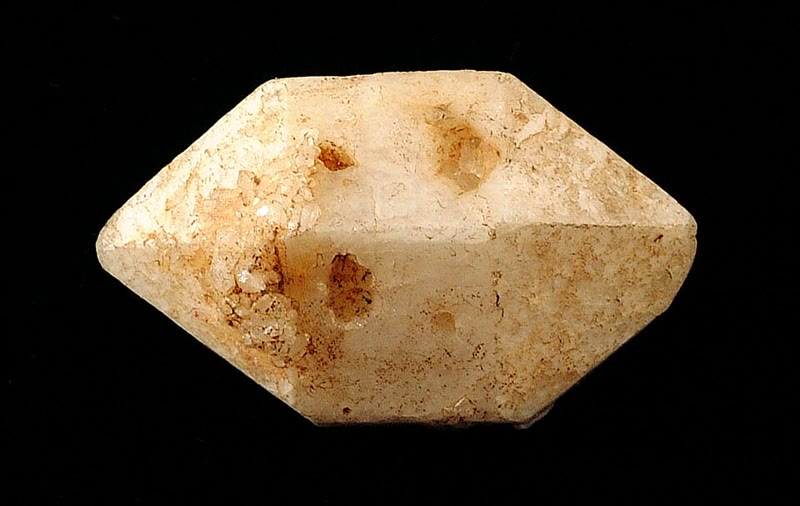
\includegraphics[height=2.75cm]{images/book2/g11-geodil-quartz.jpg}\hfill
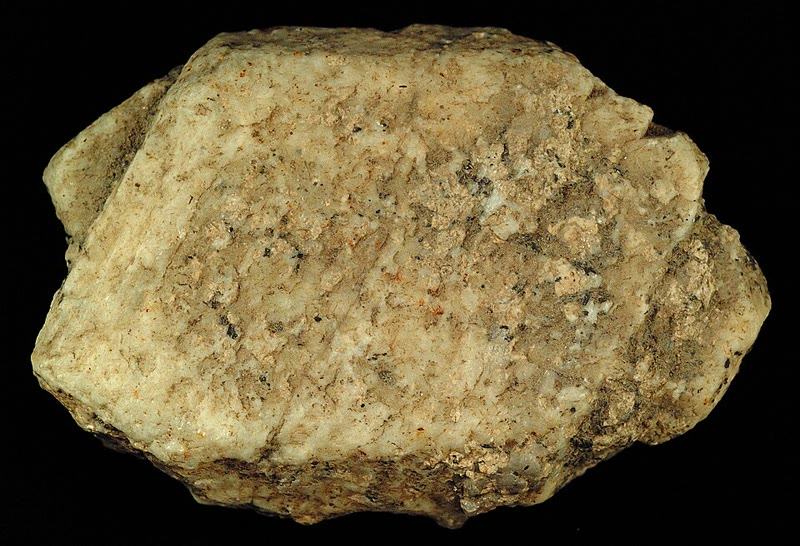
\includegraphics[height=2.75cm]{images/book2/g11-geodil-orthoclase.jpg}\hfill
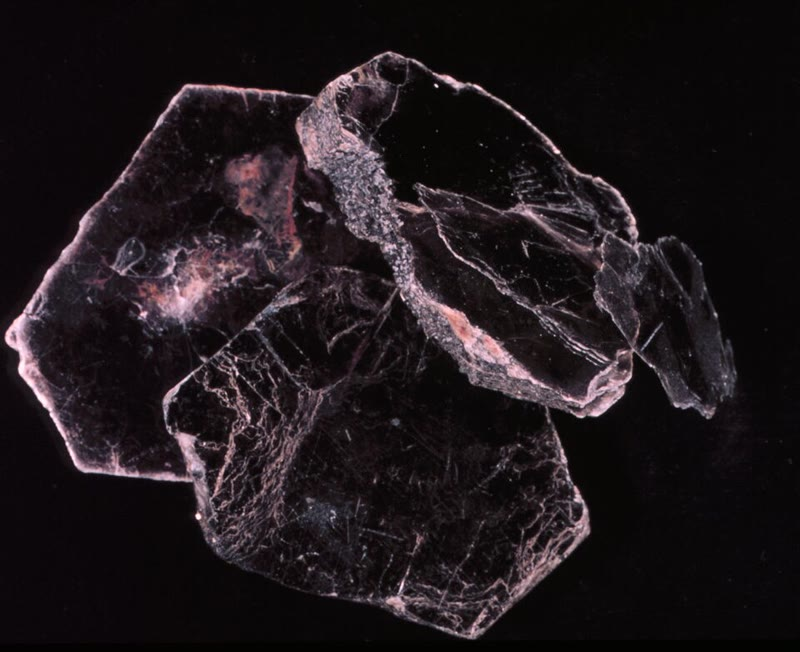
\includegraphics[height=2.75cm]{images/book2/g11-geodil-biotite.jpg}\hfill
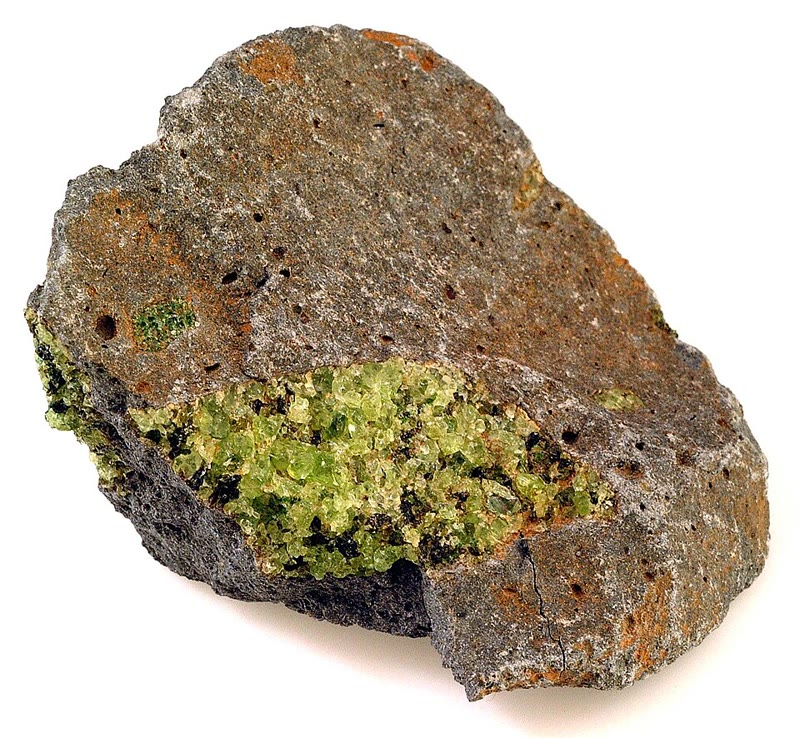
\includegraphics[height=2.75cm]{images/book2/g11-geodil-olivine.jpg}

{\small Empat mineral pembentuk batuan. Dari kiri ke kanan: kristal kuarsa,
prisma bersisi enam yang berujung runcing di kedua ujungnya, panjangnya sekitar
\qty{5}{cm}; feldspar ortoklas, dua kristal yang tumbuh bersatu, sekitar
\qty{7}{cm}; lempeng-lempeng mika biotit bersisi enam, sekitar \qty{6}{cm}, yang
terbelah menjadi lembaran tipis di sepanjang \omterm{def:g11:minerals:cleavage}{belahannya} yang tunggal; butir-butir
olivin hijau dalam basalt. Foto Shannon Heinle, Darla Sondrol, Dexter Perkins,
dan Nessa Eull, Perpustakaan Citra Digital Geologi (GeoDIL) (CC0).}
\end{omfigure}
% ledger: photo:g11-quartz, photo:g11-orthoclase, photo:g11-biotite, photo:g11-olivine

\section{Silikat}

\paragraph{Dua unsur membentuk kerak.} Komposisi kimia kerak benua diketahui dari
analisis banyak batuan, yang dilaporkan sebagai persentase oksida: sekitar
\qty{60.6}{\percent} \ce{SiO2}, \qty{15.9}{\percent} \ce{Al2O3}, dan seterusnya.
Dari nilai-nilai ini, dan dari massa atom-atomnya, massa setiap unsur dapat
dihitung. Oksigen membentuk \qty{46}{\percent} massa kerak benua dan silikon
\qty{28}{\percent}: dua unsur, sekitar tiga perempat massanya. Bersama enam logam
--- aluminium, besi, kalsium, magnesium, natrium, dan kalium --- keduanya
membentuk lebih dari \qty{99}{\percent} massa itu.
% ledger: rg14:crust, ciaaw:O, ciaaw:Si, ciaaw:Al, ciaaw:Fe, ciaaw:Ca, ciaaw:Mg, ciaaw:Na, ciaaw:K, ciaaw:Ti, ciaaw:Mn, ciaaw:P
% values (mineral_density.py): bulk_O 46.36, bulk_Si 28.30, O+Si 74.66, eight elements 99.43

\begin{omfigure}
\begin{tikzpicture}
\begin{axis}[omrecord, width=0.82\linewidth, height=5.6cm, ybar, bar width=14pt,
  ymin=0, ymax=55, xtick=data, enlarge x limits=0.06,
  xticklabels from table={figdata/out/grade-11-mineral_density-elements.dat}{symbol},
  ylabel={bagian massa (\unit{\percent})},
  nodes near coords, every node near coord/.append style={font=\scriptsize, /pgf/number format/.cd, fixed, precision=1},
  xmajorgrids=false]
% computed in figdata/grade-11/mineral_density.py; ledger: rg14:crust, ciaaw:*
\addplot[fill=omDef!55, draw=omDef] table[x expr=\coordindex, y=frac] {figdata/out/grade-11-mineral_density-elements.dat};
\end{axis}
\end{tikzpicture}

{\small Unsur-unsur kerak benua, sebagai bagian massanya, yang dihitung dari
komposisi rata-ratanya dalam oksida (Rudnick dan Gao, 2014). Oksigen dan silikon
saja membentuk sekitar tiga perempat massanya.}
\end{omfigure}

\paragraph{Tetrahedron silikon--oksigen.} Atom silikon itu kecil, dan empat atom
oksigen muat di sekelilingnya, di sudut-sudut sebuah tetrahedron, yaitu limas
dengan empat bidang segitiga. Gugus itu memuat satu ion silikon \ce{Si^4+} dan
empat ion oksigen \ce{O^2-}: gugus itu bermuatan $4 - 4 \times 2 = -4$, yang
harus diseimbangkan oleh ion-ion lain --- atau oleh tetrahedron-tetrahedron lain.

\begin{definition}[Silikat; tetrahedron silikon--oksigen]\label{def:g11:minerals:silicate}
Yang disebut \emph{tetrahedron silikon--oksigen}\index{tetrahedron silikon--oksigen}
adalah gugus \ce{SiO4} yang dibentuk oleh satu atom silikon dan empat atom
oksigen di sekelilingnya, di sudut-sudut sebuah tetrahedron. Yang disebut
\emph{silikat}\index{silikat} adalah mineral yang tersusun dari
tetrahedron-tetrahedron silikon--oksigen, yang terpisah atau saling terhubung
melalui sudut-sudut yang dipakai bersama.
\end{definition}
% ledger: tulane:silicates

Tetrahedron-tetrahedron saling terhubung dengan memakai oksigen bersama: sudut
satu tetrahedron adalah sudut tetrahedron berikutnya. Banyaknya sudut yang dipakai
bersama oleh setiap tetrahedron menentukan struktur \omterm{def:g11:minerals:silicate}{silikat} itu, dan rumusnya.
\begin{itemize}
  \item \emph{Tetrahedron terpisah}, yang tidak memakai sudut bersama, yang
        diikat satu sama lain oleh ion-ion logam di antaranya: olivin,
        \ce{(Mg,Fe)2SiO4}.
  \item \emph{Rantai tunggal}, dengan setiap tetrahedron memakai dua sudut
        bersama dengan tetangganya: piroksen.
  \item \emph{Rantai ganda}, dua rantai tunggal yang bergandengan
        berdampingan, dengan tetrahedron yang memakai dua atau tiga sudut
        bersama secara bergantian: amfibol.
  \item \emph{Lembaran}, dengan setiap tetrahedron memakai tiga sudut bersama:
        mika, dan \omterm{def:g10:soil-formation:clay}{mineral-mineral lempung} dalam tanah
        (\cref{ch:g10:soil-formation}).
  \item \emph{Kerangka}, dengan setiap tetrahedron memakai keempat sudutnya
        bersama, ke tiga arah ruang: kuarsa, \ce{SiO2}, dan --- dengan aluminium
        menggantikan sebagian silikon --- feldspar.
\end{itemize}
% ledger: tulane:silicates

\begin{omfigure}
\begin{tikzpicture}[font=\footnotesize]
  % coordinates generated once by a small script (scratch, not kept): kagome net of side 0.62 cm,
  % a regular tetrahedron in perspective, and a framework piece of five tetrahedra (painter's order)
  % (a) one SiO4 tetrahedron, drawn in perspective; the silicon (black) at its centre
  \fill[omDef!12] (2.300,2.979) -- (1.927,1.372) -- (1.221,0.629) -- (3.752,0.820) -- cycle;
  \draw[densely dashed, omDef!60, line width=0.6pt] (2.300,2.979) -- (1.927,1.372);
  \draw[omDef!70!black, line width=0.6pt] (2.300,2.979) -- (1.221,0.629);
  \draw[omDef!70!black, line width=0.6pt] (2.300,2.979) -- (3.752,0.820);
  \draw[densely dashed, omDef!60, line width=0.6pt] (1.927,1.372) -- (1.221,0.629);
  \draw[densely dashed, omDef!60, line width=0.6pt] (1.927,1.372) -- (3.752,0.820);
  \draw[omDef!70!black, line width=0.6pt] (1.221,0.629) -- (3.752,0.820);
  \draw[black!55, line width=0.4pt] (2.300,1.450) -- (2.300,2.979);
  \draw[black!55, line width=0.4pt] (2.300,1.450) -- (1.927,1.372);
  \draw[black!55, line width=0.4pt] (2.300,1.450) -- (1.221,0.629);
  \draw[black!55, line width=0.4pt] (2.300,1.450) -- (3.752,0.820);
  \fill[black] (2.300,1.450) circle (2.2pt);
  \filldraw[fill=omThm!35, draw=omThm!80!black, line width=0.4pt] (2.300,2.979) circle (4.2pt);
  \filldraw[fill=omThm!35, draw=omThm!80!black, line width=0.4pt] (1.927,1.372) circle (4.2pt);
  \filldraw[fill=omThm!35, draw=omThm!80!black, line width=0.4pt] (1.221,0.629) circle (4.2pt);
  \filldraw[fill=omThm!35, draw=omThm!80!black, line width=0.4pt] (3.752,0.820) circle (4.2pt);
  % coordinates for labels: Si 2.300,1.450; apex 2.300,2.979
  % (b) isolated tetrahedra (olivine)
  \filldraw[fill=omDef!22, draw=omDef!70!black, line width=0.5pt] (6.200,0.900) -- (6.820,0.900) -- (6.510,1.437) -- cycle;
  \fill[black] (6.510,1.079) circle (0.9pt);
  \filldraw[fill=omDef!22, draw=omDef!70!black, line width=0.5pt] (8.370,1.437) -- (8.990,1.437) -- (8.680,1.974) -- cycle;
  \fill[black] (8.680,1.616) circle (0.9pt);
  \filldraw[fill=omDef!22, draw=omDef!70!black, line width=0.5pt] (8.060,1.974) -- (7.750,2.511) -- (8.370,2.511) -- cycle;
  \fill[black] (8.060,2.332) circle (0.9pt);
  \filldraw[fill=omDef!22, draw=omDef!70!black, line width=0.5pt] (8.990,0.363) -- (9.610,0.363) -- (9.300,0.900) -- cycle;
  \fill[black] (9.300,0.542) circle (0.9pt);
  \filldraw[fill=omDef!22, draw=omDef!70!black, line width=0.5pt] (9.920,1.974) -- (9.610,2.511) -- (10.230,2.511) -- cycle;
  \fill[black] (9.920,2.332) circle (0.9pt);
  \filldraw[fill=omThm!35, draw=omThm!80!black, line width=0.4pt] (6.200,0.900) circle (1.9pt);
  \filldraw[fill=omThm!35, draw=omThm!80!black, line width=0.4pt] (6.510,1.437) circle (1.9pt);
  \filldraw[fill=omThm!35, draw=omThm!80!black, line width=0.4pt] (6.820,0.900) circle (1.9pt);
  \filldraw[fill=omThm!35, draw=omThm!80!black, line width=0.4pt] (7.750,2.511) circle (1.9pt);
  \filldraw[fill=omThm!35, draw=omThm!80!black, line width=0.4pt] (8.060,1.974) circle (1.9pt);
  \filldraw[fill=omThm!35, draw=omThm!80!black, line width=0.4pt] (8.370,2.511) circle (1.9pt);
  \filldraw[fill=omThm!35, draw=omThm!80!black, line width=0.4pt] (8.370,1.437) circle (1.9pt);
  \filldraw[fill=omThm!35, draw=omThm!80!black, line width=0.4pt] (8.680,1.974) circle (1.9pt);
  \filldraw[fill=omThm!35, draw=omThm!80!black, line width=0.4pt] (8.990,1.437) circle (1.9pt);
  \filldraw[fill=omThm!35, draw=omThm!80!black, line width=0.4pt] (9.610,2.511) circle (1.9pt);
  \filldraw[fill=omThm!35, draw=omThm!80!black, line width=0.4pt] (8.990,0.363) circle (1.9pt);
  \filldraw[fill=omThm!35, draw=omThm!80!black, line width=0.4pt] (9.300,0.900) circle (1.9pt);
  \filldraw[fill=omThm!35, draw=omThm!80!black, line width=0.4pt] (9.920,1.974) circle (1.9pt);
  \filldraw[fill=omThm!35, draw=omThm!80!black, line width=0.4pt] (10.230,2.511) circle (1.9pt);
  \filldraw[fill=omThm!35, draw=omThm!80!black, line width=0.4pt] (9.610,0.363) circle (1.9pt);
  % (c) single chain (pyroxenes)
  \filldraw[fill=omDef!22, draw=omDef!70!black, line width=0.5pt] (11.400,1.600) -- (12.020,1.600) -- (11.710,2.137) -- cycle;
  \fill[black] (11.710,1.779) circle (0.9pt);
  \filldraw[fill=omDef!22, draw=omDef!70!black, line width=0.5pt] (12.330,1.063) -- (12.020,1.600) -- (12.640,1.600) -- cycle;
  \fill[black] (12.330,1.421) circle (0.9pt);
  \filldraw[fill=omDef!22, draw=omDef!70!black, line width=0.5pt] (12.640,1.600) -- (13.260,1.600) -- (12.950,2.137) -- cycle;
  \fill[black] (12.950,1.779) circle (0.9pt);
  \filldraw[fill=omDef!22, draw=omDef!70!black, line width=0.5pt] (13.570,1.063) -- (13.260,1.600) -- (13.880,1.600) -- cycle;
  \fill[black] (13.570,1.421) circle (0.9pt);
  \filldraw[fill=omDef!22, draw=omDef!70!black, line width=0.5pt] (13.880,1.600) -- (14.500,1.600) -- (14.190,2.137) -- cycle;
  \fill[black] (14.190,1.779) circle (0.9pt);
  \filldraw[fill=omDef!22, draw=omDef!70!black, line width=0.5pt] (14.810,1.063) -- (14.500,1.600) -- (15.120,1.600) -- cycle;
  \fill[black] (14.810,1.421) circle (0.9pt);
  \filldraw[fill=omDef!22, draw=omDef!70!black, line width=0.5pt] (15.120,1.600) -- (15.740,1.600) -- (15.430,2.137) -- cycle;
  \fill[black] (15.430,1.779) circle (0.9pt);
  \filldraw[fill=omThm!35, draw=omThm!80!black, line width=0.4pt] (11.400,1.600) circle (1.9pt);
  \filldraw[fill=omThm!35, draw=omThm!80!black, line width=0.4pt] (11.710,2.137) circle (1.9pt);
  \filldraw[fill=omThm!35, draw=omThm!80!black, line width=0.4pt] (12.020,1.600) circle (1.9pt);
  \filldraw[fill=omThm!35, draw=omThm!80!black, line width=0.4pt] (12.330,1.063) circle (1.9pt);
  \filldraw[fill=omThm!35, draw=omThm!80!black, line width=0.4pt] (12.640,1.600) circle (1.9pt);
  \filldraw[fill=omThm!35, draw=omThm!80!black, line width=0.4pt] (12.950,2.137) circle (1.9pt);
  \filldraw[fill=omThm!35, draw=omThm!80!black, line width=0.4pt] (13.260,1.600) circle (1.9pt);
  \filldraw[fill=omThm!35, draw=omThm!80!black, line width=0.4pt] (13.570,1.063) circle (1.9pt);
  \filldraw[fill=omThm!35, draw=omThm!80!black, line width=0.4pt] (13.880,1.600) circle (1.9pt);
  \filldraw[fill=omThm!35, draw=omThm!80!black, line width=0.4pt] (14.190,2.137) circle (1.9pt);
  \filldraw[fill=omThm!35, draw=omThm!80!black, line width=0.4pt] (14.500,1.600) circle (1.9pt);
  \filldraw[fill=omThm!35, draw=omThm!80!black, line width=0.4pt] (14.810,1.063) circle (1.9pt);
  \filldraw[fill=omThm!35, draw=omThm!80!black, line width=0.4pt] (15.120,1.600) circle (1.9pt);
  \filldraw[fill=omThm!35, draw=omThm!80!black, line width=0.4pt] (15.430,2.137) circle (1.9pt);
  \filldraw[fill=omThm!35, draw=omThm!80!black, line width=0.4pt] (15.740,1.600) circle (1.9pt);
  % (d) double chain (amphiboles)
  \filldraw[fill=omDef!22, draw=omDef!70!black, line width=0.5pt] (0.600,-3.550) -- (1.220,-3.550) -- (0.910,-3.013) -- cycle;
  \fill[black] (0.910,-3.371) circle (0.9pt);
  \filldraw[fill=omDef!22, draw=omDef!70!black, line width=0.5pt] (1.530,-4.087) -- (1.220,-3.550) -- (1.840,-3.550) -- cycle;
  \fill[black] (1.530,-3.729) circle (0.9pt);
  \filldraw[fill=omDef!22, draw=omDef!70!black, line width=0.5pt] (1.840,-3.550) -- (2.460,-3.550) -- (2.150,-3.013) -- cycle;
  \fill[black] (2.150,-3.371) circle (0.9pt);
  \filldraw[fill=omDef!22, draw=omDef!70!black, line width=0.5pt] (2.770,-4.087) -- (2.460,-3.550) -- (3.080,-3.550) -- cycle;
  \fill[black] (2.770,-3.729) circle (0.9pt);
  \filldraw[fill=omDef!22, draw=omDef!70!black, line width=0.5pt] (3.080,-3.550) -- (3.700,-3.550) -- (3.390,-3.013) -- cycle;
  \fill[black] (3.390,-3.371) circle (0.9pt);
  \filldraw[fill=omDef!22, draw=omDef!70!black, line width=0.5pt] (4.010,-4.087) -- (3.700,-3.550) -- (4.320,-3.550) -- cycle;
  \fill[black] (4.010,-3.729) circle (0.9pt);
  \filldraw[fill=omDef!22, draw=omDef!70!black, line width=0.5pt] (4.320,-3.550) -- (4.940,-3.550) -- (4.630,-3.013) -- cycle;
  \fill[black] (4.630,-3.371) circle (0.9pt);
  \filldraw[fill=omDef!22, draw=omDef!70!black, line width=0.5pt] (0.910,-3.013) -- (0.600,-2.476) -- (1.220,-2.476) -- cycle;
  \fill[black] (0.910,-2.655) circle (0.9pt);
  \filldraw[fill=omDef!22, draw=omDef!70!black, line width=0.5pt] (1.220,-2.476) -- (1.840,-2.476) -- (1.530,-1.939) -- cycle;
  \fill[black] (1.530,-2.297) circle (0.9pt);
  \filldraw[fill=omDef!22, draw=omDef!70!black, line width=0.5pt] (2.150,-3.013) -- (1.840,-2.476) -- (2.460,-2.476) -- cycle;
  \fill[black] (2.150,-2.655) circle (0.9pt);
  \filldraw[fill=omDef!22, draw=omDef!70!black, line width=0.5pt] (2.460,-2.476) -- (3.080,-2.476) -- (2.770,-1.939) -- cycle;
  \fill[black] (2.770,-2.297) circle (0.9pt);
  \filldraw[fill=omDef!22, draw=omDef!70!black, line width=0.5pt] (3.390,-3.013) -- (3.080,-2.476) -- (3.700,-2.476) -- cycle;
  \fill[black] (3.390,-2.655) circle (0.9pt);
  \filldraw[fill=omDef!22, draw=omDef!70!black, line width=0.5pt] (3.700,-2.476) -- (4.320,-2.476) -- (4.010,-1.939) -- cycle;
  \fill[black] (4.010,-2.297) circle (0.9pt);
  \filldraw[fill=omDef!22, draw=omDef!70!black, line width=0.5pt] (4.630,-3.013) -- (4.320,-2.476) -- (4.940,-2.476) -- cycle;
  \fill[black] (4.630,-2.655) circle (0.9pt);
  \filldraw[fill=omThm!35, draw=omThm!80!black, line width=0.4pt] (0.600,-2.476) circle (1.9pt);
  \filldraw[fill=omThm!35, draw=omThm!80!black, line width=0.4pt] (0.600,-3.550) circle (1.9pt);
  \filldraw[fill=omThm!35, draw=omThm!80!black, line width=0.4pt] (0.910,-3.013) circle (1.9pt);
  \filldraw[fill=omThm!35, draw=omThm!80!black, line width=0.4pt] (1.220,-2.476) circle (1.9pt);
  \filldraw[fill=omThm!35, draw=omThm!80!black, line width=0.4pt] (1.530,-1.939) circle (1.9pt);
  \filldraw[fill=omThm!35, draw=omThm!80!black, line width=0.4pt] (1.220,-3.550) circle (1.9pt);
  \filldraw[fill=omThm!35, draw=omThm!80!black, line width=0.4pt] (1.840,-2.476) circle (1.9pt);
  \filldraw[fill=omThm!35, draw=omThm!80!black, line width=0.4pt] (1.530,-4.087) circle (1.9pt);
  \filldraw[fill=omThm!35, draw=omThm!80!black, line width=0.4pt] (1.840,-3.550) circle (1.9pt);
  \filldraw[fill=omThm!35, draw=omThm!80!black, line width=0.4pt] (2.150,-3.013) circle (1.9pt);
  \filldraw[fill=omThm!35, draw=omThm!80!black, line width=0.4pt] (2.460,-2.476) circle (1.9pt);
  \filldraw[fill=omThm!35, draw=omThm!80!black, line width=0.4pt] (2.770,-1.939) circle (1.9pt);
  \filldraw[fill=omThm!35, draw=omThm!80!black, line width=0.4pt] (2.460,-3.550) circle (1.9pt);
  \filldraw[fill=omThm!35, draw=omThm!80!black, line width=0.4pt] (3.080,-2.476) circle (1.9pt);
  \filldraw[fill=omThm!35, draw=omThm!80!black, line width=0.4pt] (2.770,-4.087) circle (1.9pt);
  \filldraw[fill=omThm!35, draw=omThm!80!black, line width=0.4pt] (3.080,-3.550) circle (1.9pt);
  \filldraw[fill=omThm!35, draw=omThm!80!black, line width=0.4pt] (3.390,-3.013) circle (1.9pt);
  \filldraw[fill=omThm!35, draw=omThm!80!black, line width=0.4pt] (3.700,-2.476) circle (1.9pt);
  \filldraw[fill=omThm!35, draw=omThm!80!black, line width=0.4pt] (4.010,-1.939) circle (1.9pt);
  \filldraw[fill=omThm!35, draw=omThm!80!black, line width=0.4pt] (3.700,-3.550) circle (1.9pt);
  \filldraw[fill=omThm!35, draw=omThm!80!black, line width=0.4pt] (4.320,-2.476) circle (1.9pt);
  \filldraw[fill=omThm!35, draw=omThm!80!black, line width=0.4pt] (4.010,-4.087) circle (1.9pt);
  \filldraw[fill=omThm!35, draw=omThm!80!black, line width=0.4pt] (4.320,-3.550) circle (1.9pt);
  \filldraw[fill=omThm!35, draw=omThm!80!black, line width=0.4pt] (4.630,-3.013) circle (1.9pt);
  \filldraw[fill=omThm!35, draw=omThm!80!black, line width=0.4pt] (4.940,-2.476) circle (1.9pt);
  \filldraw[fill=omThm!35, draw=omThm!80!black, line width=0.4pt] (4.940,-3.550) circle (1.9pt);
  % (e) sheet (micas)
  \filldraw[fill=omDef!22, draw=omDef!70!black, line width=0.5pt] (5.900,-4.100) -- (6.520,-4.100) -- (6.210,-3.563) -- cycle;
  \fill[black] (6.210,-3.921) circle (0.9pt);
  \filldraw[fill=omDef!22, draw=omDef!70!black, line width=0.5pt] (7.140,-4.100) -- (7.760,-4.100) -- (7.450,-3.563) -- cycle;
  \fill[black] (7.450,-3.921) circle (0.9pt);
  \filldraw[fill=omDef!22, draw=omDef!70!black, line width=0.5pt] (8.380,-4.100) -- (9.000,-4.100) -- (8.690,-3.563) -- cycle;
  \fill[black] (8.690,-3.921) circle (0.9pt);
  \filldraw[fill=omDef!22, draw=omDef!70!black, line width=0.5pt] (9.620,-4.100) -- (10.240,-4.100) -- (9.930,-3.563) -- cycle;
  \fill[black] (9.930,-3.921) circle (0.9pt);
  \filldraw[fill=omDef!22, draw=omDef!70!black, line width=0.5pt] (6.210,-3.563) -- (5.900,-3.026) -- (6.520,-3.026) -- cycle;
  \fill[black] (6.210,-3.205) circle (0.9pt);
  \filldraw[fill=omDef!22, draw=omDef!70!black, line width=0.5pt] (7.450,-3.563) -- (7.140,-3.026) -- (7.760,-3.026) -- cycle;
  \fill[black] (7.450,-3.205) circle (0.9pt);
  \filldraw[fill=omDef!22, draw=omDef!70!black, line width=0.5pt] (8.690,-3.563) -- (8.380,-3.026) -- (9.000,-3.026) -- cycle;
  \fill[black] (8.690,-3.205) circle (0.9pt);
  \filldraw[fill=omDef!22, draw=omDef!70!black, line width=0.5pt] (9.930,-3.563) -- (9.620,-3.026) -- (10.240,-3.026) -- cycle;
  \fill[black] (9.930,-3.205) circle (0.9pt);
  \filldraw[fill=omDef!22, draw=omDef!70!black, line width=0.5pt] (6.520,-3.026) -- (7.140,-3.026) -- (6.830,-2.489) -- cycle;
  \fill[black] (6.830,-2.847) circle (0.9pt);
  \filldraw[fill=omDef!22, draw=omDef!70!black, line width=0.5pt] (7.760,-3.026) -- (8.380,-3.026) -- (8.070,-2.489) -- cycle;
  \fill[black] (8.070,-2.847) circle (0.9pt);
  \filldraw[fill=omDef!22, draw=omDef!70!black, line width=0.5pt] (9.000,-3.026) -- (9.620,-3.026) -- (9.310,-2.489) -- cycle;
  \fill[black] (9.310,-2.847) circle (0.9pt);
  \filldraw[fill=omDef!22, draw=omDef!70!black, line width=0.5pt] (6.830,-2.489) -- (6.520,-1.952) -- (7.140,-1.952) -- cycle;
  \fill[black] (6.830,-2.131) circle (0.9pt);
  \filldraw[fill=omDef!22, draw=omDef!70!black, line width=0.5pt] (8.070,-2.489) -- (7.760,-1.952) -- (8.380,-1.952) -- cycle;
  \fill[black] (8.070,-2.131) circle (0.9pt);
  \filldraw[fill=omDef!22, draw=omDef!70!black, line width=0.5pt] (9.310,-2.489) -- (9.000,-1.952) -- (9.620,-1.952) -- cycle;
  \fill[black] (9.310,-2.131) circle (0.9pt);
  \filldraw[fill=omDef!22, draw=omDef!70!black, line width=0.5pt] (5.900,-1.952) -- (6.520,-1.952) -- (6.210,-1.415) -- cycle;
  \fill[black] (6.210,-1.773) circle (0.9pt);
  \filldraw[fill=omDef!22, draw=omDef!70!black, line width=0.5pt] (7.140,-1.952) -- (7.760,-1.952) -- (7.450,-1.415) -- cycle;
  \fill[black] (7.450,-1.773) circle (0.9pt);
  \filldraw[fill=omDef!22, draw=omDef!70!black, line width=0.5pt] (8.380,-1.952) -- (9.000,-1.952) -- (8.690,-1.415) -- cycle;
  \fill[black] (8.690,-1.773) circle (0.9pt);
  \filldraw[fill=omDef!22, draw=omDef!70!black, line width=0.5pt] (9.620,-1.952) -- (10.240,-1.952) -- (9.930,-1.415) -- cycle;
  \fill[black] (9.930,-1.773) circle (0.9pt);
  \filldraw[fill=omThm!35, draw=omThm!80!black, line width=0.4pt] (5.900,-1.952) circle (1.9pt);
  \filldraw[fill=omThm!35, draw=omThm!80!black, line width=0.4pt] (6.210,-1.415) circle (1.9pt);
  \filldraw[fill=omThm!35, draw=omThm!80!black, line width=0.4pt] (5.900,-3.026) circle (1.9pt);
  \filldraw[fill=omThm!35, draw=omThm!80!black, line width=0.4pt] (6.520,-1.952) circle (1.9pt);
  \filldraw[fill=omThm!35, draw=omThm!80!black, line width=0.4pt] (5.900,-4.100) circle (1.9pt);
  \filldraw[fill=omThm!35, draw=omThm!80!black, line width=0.4pt] (6.210,-3.563) circle (1.9pt);
  \filldraw[fill=omThm!35, draw=omThm!80!black, line width=0.4pt] (6.520,-3.026) circle (1.9pt);
  \filldraw[fill=omThm!35, draw=omThm!80!black, line width=0.4pt] (6.830,-2.489) circle (1.9pt);
  \filldraw[fill=omThm!35, draw=omThm!80!black, line width=0.4pt] (7.140,-1.952) circle (1.9pt);
  \filldraw[fill=omThm!35, draw=omThm!80!black, line width=0.4pt] (7.450,-1.415) circle (1.9pt);
  \filldraw[fill=omThm!35, draw=omThm!80!black, line width=0.4pt] (6.520,-4.100) circle (1.9pt);
  \filldraw[fill=omThm!35, draw=omThm!80!black, line width=0.4pt] (7.140,-3.026) circle (1.9pt);
  \filldraw[fill=omThm!35, draw=omThm!80!black, line width=0.4pt] (7.760,-1.952) circle (1.9pt);
  \filldraw[fill=omThm!35, draw=omThm!80!black, line width=0.4pt] (7.140,-4.100) circle (1.9pt);
  \filldraw[fill=omThm!35, draw=omThm!80!black, line width=0.4pt] (7.450,-3.563) circle (1.9pt);
  \filldraw[fill=omThm!35, draw=omThm!80!black, line width=0.4pt] (7.760,-3.026) circle (1.9pt);
  \filldraw[fill=omThm!35, draw=omThm!80!black, line width=0.4pt] (8.070,-2.489) circle (1.9pt);
  \filldraw[fill=omThm!35, draw=omThm!80!black, line width=0.4pt] (8.380,-1.952) circle (1.9pt);
  \filldraw[fill=omThm!35, draw=omThm!80!black, line width=0.4pt] (8.690,-1.415) circle (1.9pt);
  \filldraw[fill=omThm!35, draw=omThm!80!black, line width=0.4pt] (7.760,-4.100) circle (1.9pt);
  \filldraw[fill=omThm!35, draw=omThm!80!black, line width=0.4pt] (8.380,-3.026) circle (1.9pt);
  \filldraw[fill=omThm!35, draw=omThm!80!black, line width=0.4pt] (9.000,-1.952) circle (1.9pt);
  \filldraw[fill=omThm!35, draw=omThm!80!black, line width=0.4pt] (8.380,-4.100) circle (1.9pt);
  \filldraw[fill=omThm!35, draw=omThm!80!black, line width=0.4pt] (8.690,-3.563) circle (1.9pt);
  \filldraw[fill=omThm!35, draw=omThm!80!black, line width=0.4pt] (9.000,-3.026) circle (1.9pt);
  \filldraw[fill=omThm!35, draw=omThm!80!black, line width=0.4pt] (9.310,-2.489) circle (1.9pt);
  \filldraw[fill=omThm!35, draw=omThm!80!black, line width=0.4pt] (9.620,-1.952) circle (1.9pt);
  \filldraw[fill=omThm!35, draw=omThm!80!black, line width=0.4pt] (9.930,-1.415) circle (1.9pt);
  \filldraw[fill=omThm!35, draw=omThm!80!black, line width=0.4pt] (9.000,-4.100) circle (1.9pt);
  \filldraw[fill=omThm!35, draw=omThm!80!black, line width=0.4pt] (9.620,-3.026) circle (1.9pt);
  \filldraw[fill=omThm!35, draw=omThm!80!black, line width=0.4pt] (10.240,-1.952) circle (1.9pt);
  \filldraw[fill=omThm!35, draw=omThm!80!black, line width=0.4pt] (9.620,-4.100) circle (1.9pt);
  \filldraw[fill=omThm!35, draw=omThm!80!black, line width=0.4pt] (9.930,-3.563) circle (1.9pt);
  \filldraw[fill=omThm!35, draw=omThm!80!black, line width=0.4pt] (10.240,-3.026) circle (1.9pt);
  \filldraw[fill=omThm!35, draw=omThm!80!black, line width=0.4pt] (10.240,-4.100) circle (1.9pt);
  % (f) framework: a tetrahedron sharing all four corners
  \filldraw[fill=omThm!35, draw=omThm!80!black, line width=0.4pt] (12.990,-1.963) circle (2.1pt);
  \filldraw[fill=omThm!35, draw=omThm!80!black, line width=0.4pt] (12.896,-3.062) circle (2.1pt);
  \filldraw[fill=omDef!14, draw=omDef!70!black, line width=0.45pt, fill opacity=0.85] (12.896,-3.062) -- (12.990,-1.963) -- (12.299,-2.380) -- cycle;
  \filldraw[fill=omThm!35, draw=omThm!80!black, line width=0.4pt] (15.186,-2.119) circle (2.1pt);
  \filldraw[fill=omDef!14, draw=omDef!70!black, line width=0.45pt, fill opacity=0.85] (12.896,-3.062) -- (13.398,-2.458) -- (12.990,-1.963) -- cycle;
  \filldraw[fill=omThm!35, draw=omThm!80!black, line width=0.4pt] (15.092,-3.219) circle (2.1pt);
  \fill[black] (12.896,-2.466) circle (1.1pt);
  \filldraw[fill=omDef!34, draw=omDef!70!black, line width=0.45pt, fill opacity=0.85] (13.398,-2.458) -- (12.990,-1.963) -- (12.299,-2.380) -- cycle;
  \filldraw[fill=omDef!14, draw=omDef!70!black, line width=0.45pt, fill opacity=0.85] (15.092,-3.219) -- (15.186,-2.119) -- (14.496,-2.536) -- cycle;
  \filldraw[fill=omDef!25, draw=omDef!70!black, line width=0.45pt, fill opacity=0.85] (12.896,-3.062) -- (12.299,-2.380) -- (13.398,-2.458) -- cycle;
  \filldraw[fill=omDef!14, draw=omDef!70!black, line width=0.45pt, fill opacity=0.85] (15.092,-3.219) -- (15.595,-2.614) -- (15.186,-2.119) -- cycle;
  \fill[black] (15.092,-2.622) circle (1.1pt);
  \filldraw[fill=omThm!35, draw=omThm!80!black, line width=0.4pt] (12.299,-2.380) circle (2.1pt);
  \filldraw[fill=omDef!34, draw=omDef!70!black, line width=0.45pt, fill opacity=0.85] (15.595,-2.614) -- (15.186,-2.119) -- (14.496,-2.536) -- cycle;
  \filldraw[fill=omDef!25, draw=omDef!70!black, line width=0.45pt, fill opacity=0.85] (15.092,-3.219) -- (14.496,-2.536) -- (15.595,-2.614) -- cycle;
  \filldraw[fill=omThm!35, draw=omThm!80!black, line width=0.4pt] (13.398,-2.458) circle (2.1pt);
  \filldraw[fill=omThm!35, draw=omThm!80!black, line width=0.4pt] (14.496,-2.536) circle (2.1pt);
  \filldraw[fill=omDef!14, draw=omDef!70!black, line width=0.45pt, fill opacity=0.85] (13.900,-1.853) -- (14.496,-2.536) -- (13.398,-2.458) -- cycle;
  \filldraw[fill=omThm!35, draw=omThm!80!black, line width=0.4pt] (15.595,-2.614) circle (2.1pt);
  \filldraw[fill=omDef!14, draw=omDef!70!black, line width=0.45pt, fill opacity=0.85] (13.398,-2.458) -- (13.806,-2.953) -- (14.496,-2.536) -- cycle;
  \fill[black] (13.900,-2.450) circle (1.1pt);
  \filldraw[fill=omDef!22, draw=omDef!70!black, line width=0.45pt, fill opacity=0.85] (13.900,-1.853) -- (13.398,-2.458) -- (13.806,-2.953) -- cycle;
  \filldraw[fill=omDef!37, draw=omDef!70!black, line width=0.45pt, fill opacity=0.85] (13.900,-1.853) -- (13.806,-2.953) -- (14.496,-2.536) -- cycle;
  \filldraw[fill=omThm!35, draw=omThm!80!black, line width=0.4pt] (13.994,-0.754) circle (2.1pt);
  \filldraw[fill=omThm!35, draw=omThm!80!black, line width=0.4pt] (13.900,-1.853) circle (2.1pt);
  \filldraw[fill=omThm!35, draw=omThm!80!black, line width=0.4pt] (13.806,-2.953) circle (2.1pt);
  \filldraw[fill=omDef!14, draw=omDef!70!black, line width=0.45pt, fill opacity=0.85] (13.900,-1.853) -- (13.994,-0.754) -- (13.304,-1.171) -- cycle;
  \filldraw[fill=omDef!14, draw=omDef!70!black, line width=0.45pt, fill opacity=0.85] (13.900,-1.853) -- (14.402,-1.249) -- (13.994,-0.754) -- cycle;
  \filldraw[fill=omThm!35, draw=omThm!80!black, line width=0.4pt] (13.712,-4.053) circle (2.1pt);
  \fill[black] (13.900,-1.256) circle (1.1pt);
  \filldraw[fill=omDef!14, draw=omDef!70!black, line width=0.45pt, fill opacity=0.85] (13.712,-4.053) -- (13.806,-2.953) -- (13.116,-3.370) -- cycle;
  \filldraw[fill=omDef!34, draw=omDef!70!black, line width=0.45pt, fill opacity=0.85] (14.402,-1.249) -- (13.994,-0.754) -- (13.304,-1.171) -- cycle;
  \filldraw[fill=omDef!14, draw=omDef!70!black, line width=0.45pt, fill opacity=0.85] (13.712,-4.053) -- (14.214,-3.448) -- (13.806,-2.953) -- cycle;
  \filldraw[fill=omDef!25, draw=omDef!70!black, line width=0.45pt, fill opacity=0.85] (13.900,-1.853) -- (13.304,-1.171) -- (14.402,-1.249) -- cycle;
  \fill[black] (13.712,-3.456) circle (1.1pt);
  \filldraw[fill=omThm!35, draw=omThm!80!black, line width=0.4pt] (13.304,-1.171) circle (2.1pt);
  \filldraw[fill=omDef!34, draw=omDef!70!black, line width=0.45pt, fill opacity=0.85] (14.214,-3.448) -- (13.806,-2.953) -- (13.116,-3.370) -- cycle;
  \filldraw[fill=omDef!25, draw=omDef!70!black, line width=0.45pt, fill opacity=0.85] (13.712,-4.053) -- (13.116,-3.370) -- (14.214,-3.448) -- cycle;
  \filldraw[fill=omThm!35, draw=omThm!80!black, line width=0.4pt] (14.402,-1.249) circle (2.1pt);
  \filldraw[fill=omThm!35, draw=omThm!80!black, line width=0.4pt] (13.116,-3.370) circle (2.1pt);
  \filldraw[fill=omThm!35, draw=omThm!80!black, line width=0.4pt] (14.214,-3.448) circle (2.1pt);
  % labels
  \draw[black!60] (2.30,2.98) -- (3.35,3.25); \node[anchor=west] at (3.35,3.25) {oksigen};
  \draw[black!60] (2.30,1.45) -- (3.55,2.15); \node[anchor=west] at (3.55,2.15) {silikon};
  \node[align=center] at (2.3,-0.15) {(a) satu tetrahedron, \ce{SiO4}};
  \node[align=center] at (8.2,-0.15) {(b) tetrahedron terpisah:\\olivin};
  \node[align=center] at (13.5,-0.15) {(c) rantai tunggal:\\piroksen};
  \node[align=center] at (2.75,-4.85) {(d) rantai ganda:\\amfibol};
  \node[align=center] at (8.1,-4.85) {(e) lembaran:\\mika};
  \node[align=center] at (13.9,-4.85) {(f) kerangka:\\kuarsa, feldspar};
\end{tikzpicture}

{\small (a) \omterm{def:g11:minerals:silicate}{Tetrahedron silikon--oksigen}: satu atom silikon (hitam) dan empat
atom oksigen (merah muda) di sudut-sudut sebuah tetrahedron. (b)--(e)
Tetrahedron-tetrahedron dilihat dari atas, masing-masing sebagai segitiga:
lingkaran-lingkarannya adalah oksigen alasnya, titiknya adalah silikon, di bawah
oksigen keempat; dua segitiga yang bertemu di satu sudut memakai oksigen itu
bersama. (f) Dalam kerangka setiap sudut dipakai bersama, dalam tiga dimensi: di
sini satu tetrahedron dan keempat tetangganya. Gambar, tidak berskala.}
\end{omfigure}
% ledger: tulane:silicates

\begin{proposition}[Menghitung oksigen]\label{prop:g11:minerals:sharing}
Dalam \omterm{def:g11:minerals:silicate}{silikat} yang setiap tetrahedronnya memakai $n$ sudutnya bersama dengan
tetrahedron lain, terdapat $4 - n/2$ atom oksigen untuk setiap atom silikon.
Tetrahedron terpisah memberikan \ce{SiO4}, rantai tunggal \ce{SiO3}, lembaran
\ce{Si2O5}, dan kerangka \ce{SiO2}.
\end{proposition}

\begin{proof}
Setiap tetrahedron mempunyai satu silikon dan empat sudut. Sudut yang tidak
dipakai bersama hanya dimiliki tetrahedron ini dan dihitung sebagai satu oksigen;
sudut yang dipakai bersama dimiliki dua tetrahedron dan dihitung sebagai setengah
oksigen pada masing-masing. Dengan $n$ sudut yang dipakai bersama, sebuah
tetrahedron memiliki $(4 - n) + n/2 = 4 - n/2$ oksigen.
Untuk $n = 0$, $2$, $3$, dan $4$ hasilnya $4$, $3$, $5/2$, dan $2$ oksigen
per silikon: \ce{SiO4}, \ce{SiO3}, \ce{Si2O5}, dan \ce{SiO2}.
\end{proof}

Rumus-rumus mineral membenarkan hal ini. Piroksen augit mengandung
\ce{(Si,Al)2O6}, yaitu dua kali \ce{SiO3}, dan mika biotit \ce{AlSi3O10},
empat tetrahedron untuk sepuluh oksigen, dua kali \ce{Si2O5}; dalam feldspar,
empat tetrahedron memuat delapan oksigen, empat kali \ce{SiO2}, tepat seperti
pada kuarsa. Namun muatannya berbeda. Kuarsa netral: dalam kerangka, setiap
oksigen dipakai bersama, dan muatan silikon dan oksigen seimbang. Pada
struktur-struktur lain, oksigen yang tidak dipakai bersama membawa kelebihan
muatan negatif, yang diseimbangkan oleh ion-ion logam --- magnesium dan besi pada
olivin, kalium pada ortoklas, tempat satu ion aluminium \ce{Al^3+} yang
menggantikan satu ion silikon \ce{Si^4+} menyisakan satu muatan yang harus
diseimbangkan.
% ledger: wm:densities (formulas)

\begin{definition}[Silikat pembentuk batuan]\label{def:g11:minerals:rock-forming}
Yang disebut \emph{silikat pembentuk batuan}\index{silikat pembentuk batuan}
adalah enam golongan mineral \omterm{def:g11:minerals:silicate}{silikat} yang membentuk sebagian besar batuan beku
dan metamorf yang umum: olivin, piroksen, amfibol, mika, feldspar, dan kuarsa.
Feldspar terdiri atas dua jenis: \emph{feldspar kalium}, seperti ortoklas, dan
\emph{plagioklas}, deret feldspar yang mengandung natrium dan kalsium.
\end{definition}
% ledger: tulane:silicates, wm:densities

\begin{center}
\small
\renewcommand{\arraystretch}{1.25}
\begin{tabular}{|l|l|l|c|}
\hline
\textbf{golongan (contoh)} & \textbf{struktur} & \textbf{rumus} & \textbf{massa jenis} \\
 & & & (\unit{g/cm^3}) \\
\hline
olivin & tetrahedron terpisah & \ce{(Mg,Fe)2SiO4} & 3.32 \\
piroksen (augit) & rantai tunggal & \ce{(Ca,Na)(Mg,Fe,Al,Ti)(Si,Al)2O6} & 3.4 \\
amfibol (hornblende) & rantai ganda & \ce{Ca2[Mg4(Al,Fe)]Si7AlO22(OH)2} & 3.23 \\
mika (biotit) & lembaran & \ce{K(Mg,Fe)3AlSi3O10(OH,F)2} & 3.09 \\
mika (muskovit) & lembaran & \ce{KAl2(Si3Al)O10(OH,F)2} & 2.82 \\
feldspar kalium (ortoklas) & kerangka & \ce{KAlSi3O8} & 2.56 \\
plagioklas (oligoklas) & kerangka & \ce{(Na,Ca)(Si,Al)4O8} & 2.65 \\
kuarsa & kerangka & \ce{SiO2} & 2.62 \\
\hline
\end{tabular}

\smallskip
{\footnotesize \omterm{def:g11:minerals:rock-forming}{Silikat pembentuk batuan}. Rumus dan massa jenis rata-rata dari
webmineral.com; koma di antara dua unsur di dalam kurung berarti bahwa salah
satunya dapat menempati tempat itu di dalam kristal.}
\end{center}
% ledger: wm:densities, tulane:silicates

Tabel ini memuat sebuah aturan yang berlaku di sepanjang sisa buku ini. Mineral
dengan tetrahedron terpisah dan rantai, yang kaya akan besi dan magnesium, adalah
yang paling rapat, di atas \qty{3.2}{g/cm^3}; kerangka, yang terdiri atas
silikon, aluminium, natrium, kalium, dan kalsium, adalah yang paling ringan,
sekitar \qty{2.6}{g/cm^3}. Mika terletak di antaranya. Olivin dan piroksen
membentuk \omterm{def:g11:ocean-ridges:peridotite}{peridotit} mantel; feldspar dan kuarsa, granit benua: batuan yang ringan
mengapung di atas batuan yang rapat.
% ledger: wm:densities

\section{Mineral membentuk batuan}

Sebuah batuan diperikan pertama-tama oleh mineral-mineralnya dan proporsinya. Tiga
batuan yang telah dijumpai pada bab-bab sebelumnya menunjukkan rentangnya:
\begin{itemize}
  \item \emph{granit}: kuarsa, feldspar kalium, dan plagioklas, dengan sedikit
        biotit atau muskovit --- batuan benua;
  \item \emph{basalt} dan \emph{\omterm{def:g11:ocean-ridges:gabbro}{gabro}}: plagioklas dan piroksen, sering dengan
        olivin --- batuan \omterm{def:g11:ocean-ridges:oceanic-lithosphere}{kerak samudra}, yang pertama berbutir halus, yang kedua
        berbutir kasar (\cref{ch:g11:igneous-rocks});
  \item \emph{\omterm{def:g11:ocean-ridges:peridotite}{peridotit}}: sebagian besar olivin, dengan piroksen --- batuan
        mantel.
\end{itemize}
% ledger: nps:granite-minerals, photo:g11-basalt-thin-section, photo:g11-olivine

\begin{omfigure}
\begin{tikzpicture}
\begin{axis}[omrecord, width=0.8\linewidth, height=6.4cm, xbar, bar width=8pt,
  xmin=2.4, xmax=3.5, ymin=-0.7, ymax=8.7, ytick={0,...,8},
  yticklabels={ortoklas, kuarsa, oligoklas, labradorit, muskovit, biotit, hornblende, olivin, augit},
  xlabel={massa jenis (\unit{g/cm^3})}, ymajorgrids=false, clip=false]
% computed in figdata/grade-11/mineral_density.py (density_order); ledger: wm:densities
\addplot[fill=omDef!45, draw=omDef] table[x=rho, y=idx] {figdata/out/grade-11-mineral_density-densities.dat};
\draw[omProp, line width=1pt, dashed] (axis cs:2.6427,-0.7) -- (axis cs:2.6427,8.7) node[above, text height=1.6ex, text depth=0.3ex, font=\scriptsize, text=omProp!80!black] {granit};
\draw[omThm, line width=1pt, dashed] (axis cs:3.0015,-0.7) -- (axis cs:3.0015,8.7) node[above, text height=1.6ex, text depth=0.3ex, font=\scriptsize, text=omThm] {basalt};
\draw[black!70, line width=1pt, dashed] (axis cs:3.34,-0.7) -- (axis cs:3.34,8.7) node[above, font=\scriptsize] {peridotit};
\end{axis}
\end{tikzpicture}

{\small Massa jenis rata-rata sembilan mineral pembentuk batuan (webmineral.com),
dan massa jenis ketiga batuan contoh pada bagian ini yang dihitung dengan
proposisi di bawah (garis putus-putus): granit dari kuarsa, feldspar, dan mika,
basalt dari plagioklas, piroksen, dan sedikit olivin, \omterm{def:g11:ocean-ridges:peridotite}{peridotit} dari olivin dan
piroksen.}
\end{omfigure}
% values (mineral_density.py): rho_granite 2.6427, rho_basalt 3.0015, rho_peridotite 3.34

Massa jenis sebuah batuan dapat diturunkan dari mineral-mineralnya. Bayangkan
sebuah blok batuan bervolume $V$, yang bagian $\phi_1$-nya terdiri atas mineral
pertama, $\phi_2$ atas mineral kedua, dan seterusnya.

\begin{proposition}[Massa jenis batuan dari mineral-mineralnya]\label{prop:g11:minerals:density}
Batuan tanpa pori, yang terdiri atas mineral-mineral bermassa jenis $\rho_1, \rho_2, \dots,
\rho_k$ yang menempati bagian $\phi_1, \phi_2, \dots, \phi_k$ volumenya
($\phi_1 + \dots + \phi_k = 1$), mempunyai massa jenis
\[
  \rho = \phi_1 \rho_1 + \phi_2 \rho_2 + \dots + \phi_k \rho_k ,
\]
yaitu rata-rata massa jenis mineral-mineralnya, yang diberi bobot menurut bagian
volumenya.
\end{proposition}

\begin{proof}
Dalam volume $V$ batuan, mineral $i$ menempati volume $\phi_i V$ dan bermassa
$\rho_i \phi_i V$. Tanpa pori, massa batuan adalah jumlah massa-massa ini,
$m = (\phi_1 \rho_1 + \dots + \phi_k \rho_k)\,V$, dan massa jenisnya adalah
$m/V$.
\end{proof}

Bagaimana bagian volume itu diukur? Pada permukaan potongan batuan yang rata,
atau pada \omterm{def:g11:minerals:thin-section}{sayatan tipis} (bagian berikutnya), dibuat kisi titik-titik yang
teratur, dan pada setiap titik dicatat mineral yang ada di bawahnya. Bila
butir-butirnya tersebar tanpa keteraturan, bagian titik yang jatuh pada sebuah
mineral menaksir bagian luas yang ditutupi mineral itu, dan itu juga bagian
volume yang diisinya: irisan tipis adalah contoh yang wajar bagi seluruh blok.
Cara ini disebut \emph{penghitungan titik}.

\begin{example}[Granit yang ringan, kaya akan kuarsa dan feldspar kalium]
Penghitungan titik memberikan \qty{35}{\percent} kuarsa (\qty{2.62}{g/cm^3}),
\qty{50}{\percent} ortoklas (\qty{2.56}{g/cm^3}), dan \qty{15}{\percent}
oligoklas (\qty{2.65}{g/cm^3}). Massa jenis batuan itu adalah
\[
  \rho = 0.35 \times 2.62 + 0.50 \times 2.56 + 0.15 \times 2.65
       = 0.917 + 1.280 + 0.398 \approx \qty{2.59}{g/cm^3}.
\]
Pengukuran membenarkan orde besaran ini: dari \num{6454} contoh batuan yang
ditimbang dari sekitar dua ratus tubuh batuan granitik di Sierra Nevada,
California, rata-ratanya \qty{2.69}{g/cm^3}, dan granit yang paling kaya akan
silika dan kalium, seperti granit ini, berada di bawah \qty{2.6}{g/cm^3}.
\end{example}
% ledger: wm:densities, usgs91:sierra

\section{Sayatan tipis}

Kaca pembesar memperlihatkan butir-butir selebar satu milimeter. Untuk melihat
butir-butir yang lebih halus, dan untuk mengenalinya dengan pasti, ahli geologi
mengamati batuan melalui mikroskop --- bukan permukaannya, melainkan menembus
batuan itu.

\begin{definition}[Sayatan tipis; mikroskop polarisasi]\label{def:g11:minerals:thin-section}
Yang disebut \emph{sayatan tipis}\index{sayatan tipis} adalah irisan batuan yang
digerinda sampai setebal \qty{0.03}{mm} dan dipasang pada kaca objek: pada tebal
ini cahaya dapat menembus kebanyakan mineral. Yang disebut \emph{mikroskop
polarisasi}\index{mikroskop polarisasi} adalah mikroskop yang dilengkapi dua
filter polarisasi, satu di bawah kaca objek dan satu di atasnya. Sayatan itu
dilihat dalam \emph{cahaya terpolarisasi bidang} dengan filter bawah saja, dan di
antara \emph{polarisator bersilang} bila filter atas ditambahkan dengan arahnya
tegak lurus pada arah filter bawah.
\end{definition}
% ledger: tulane:thin-section

\begin{omfigure}
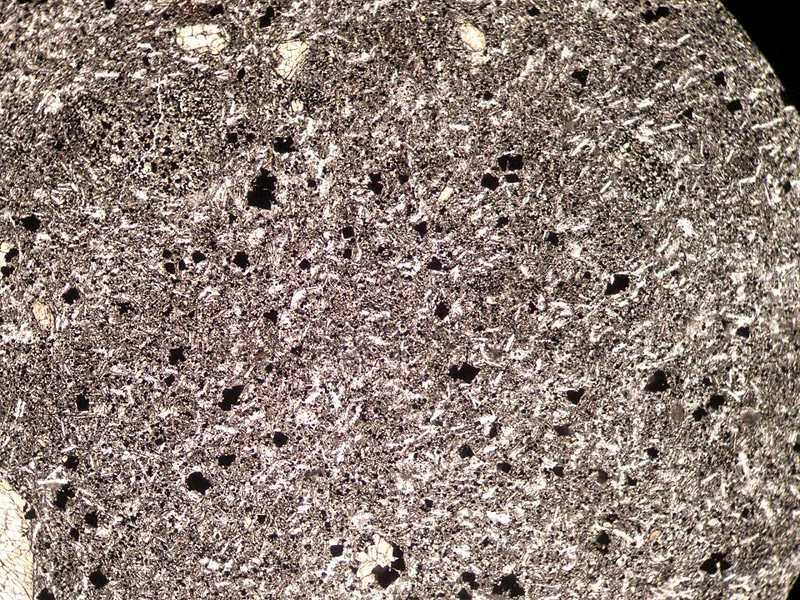
\includegraphics[height=3.6cm]{images/book2/g11-chmee2-basalt-ppl.jpg}\hfill
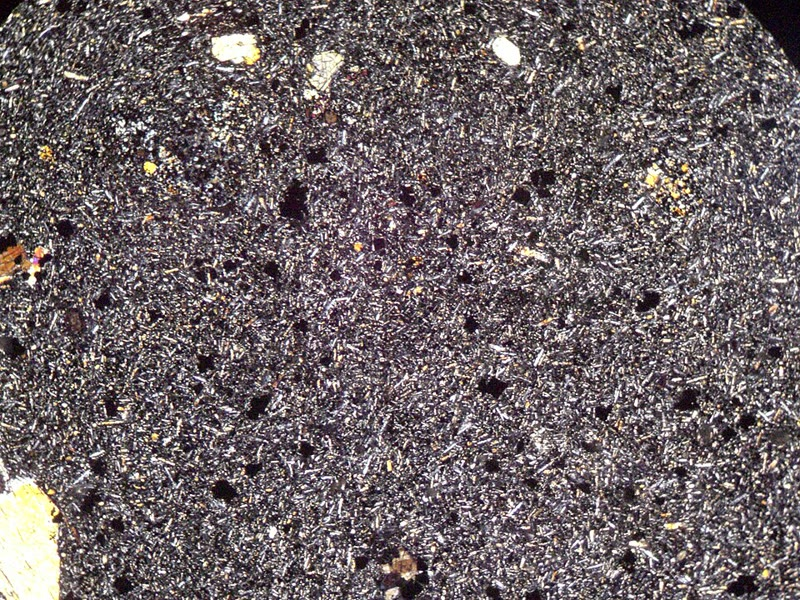
\includegraphics[height=3.6cm]{images/book2/g11-chmee2-basalt-xpl.jpg}\hfill
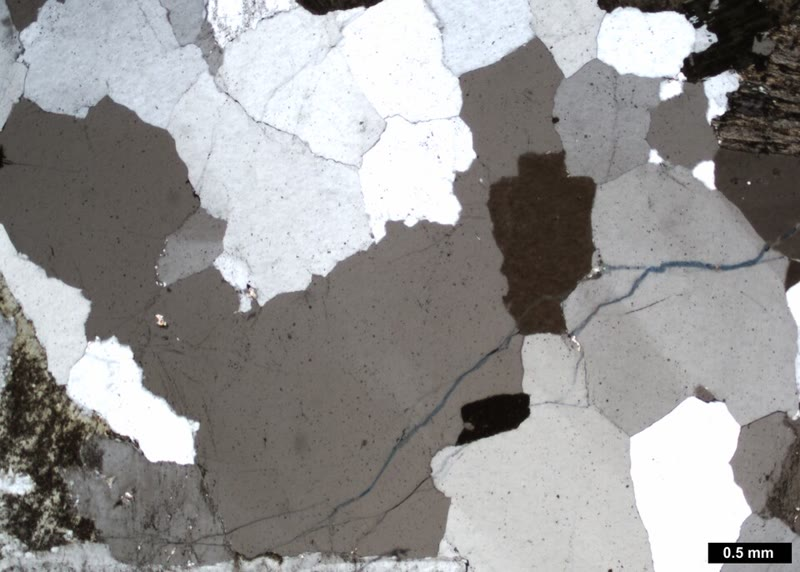
\includegraphics[height=3.6cm]{images/book2/g11-rygel-granite-xpl.jpg}

{\small Kiri dan tengah: basalt yang sama dalam \omterm{def:g11:minerals:thin-section}{sayatan tipis}, dalam cahaya
terpolarisasi bidang dan di antara polarisator bersilang. Batuan itu berbutir
halus: kristal-kristal kecil yang memanjang, sebagian besar plagioklas, dan
bintik-bintik hitam yang tidak meneruskan cahaya sama sekali pada kedua
pengamatan; di antara polarisator bersilang kristal-kristal itu menyala dalam
warna kelabu dan warna-warni. Foto
Chmee2 (CC~BY-SA~3.0). Kanan: kristal-kristal kuarsa dalam granit, di antara
polarisator bersilang, masing-masing dengan rona kelabunya sendiri (batang skala
\qty{0.5}{mm}). Foto Michael C.~Rygel (CC~BY-SA~3.0).}
\end{omfigure}
% ledger: photo:g11-basalt-thin-section, photo:g11-granite-thin-section

Dalam cahaya terpolarisasi bidang, \omterm{def:g11:minerals:thin-section}{sayatan tipis} tampak seperti jendela kaca
patri: kebanyakan mineral hampir tidak berwarna, sebagian berwarna lembut, dan
garis tepi butir-butirnya, \omterm{def:g11:minerals:cleavage}{belahannya}, dan \omterm{def:g11:minerals:habit}{habitusnya} tampak tajam. Di antara
polarisator bersilang, kedua filter, yang dipasang saling bersilangan, sendirian
tidak akan meneruskan cahaya sama sekali; kebanyakan mineral mengubah cahaya yang
menembusnya, dan tampak dalam rona kelabu atau dalam warna-warna cerah, yang
berubah ketika kaca objek diputar. Dua butir mineral yang sama dapat tampak
berbeda, karena masing-masing terpotong ke arahnya sendiri: butir-butir kuarsa
dalam granit di atas semuanya kuarsa, dalam rona yang berbeda-beda. Warna-warna
itu, bagaimana warna itu berubah, dan apa yang diungkapkannya tentang setiap
mineral adalah pokok bahasan tahun pertama di universitas; di sini, \omterm{def:g11:minerals:thin-section}{sayatan tipis}
adalah gambar batuan, yang di dalamnya setiap butir dapat dilihat, dinamai, dan
dihitung.

\section{Latihan}

\begin{exercise}[$\star$]\label{exo:g11:minerals:1}
Definisikan \omterm{def:g11:minerals:cleavage}{belahan} dan \omterm{def:g11:minerals:cleavage}{pecahan}. Mana yang diperlihatkan kuarsa, dan seperti apa
permukaan patahnya? Berapa \omterm{def:g11:minerals:cleavage}{belahan} yang dimiliki mika?
\end{exercise}

\begin{exercise}[$\star$]\label{exo:g11:minerals:2}
Mengapa warna adalah petunjuk yang buruk untuk mengenali kuarsa, tetapi cukup baik
untuk olivin? Berikan dua sifat yang lebih dapat diandalkan daripada warna.
\end{exercise}

\begin{exercise}[$\star$]\label{exo:g11:minerals:3}
Pasangkan setiap pemerian dengan sebuah mineral di antara kuarsa, ortoklas,
biotit, dan olivin: (1) butir-butir hijau dalam basalt; (2) serpih hitam yang
terkelupas menjadi lembaran tipis; (3) butir merah muda berbentuk balok dengan dua
bidang pecah yang datar, yang tergores oleh paku baja; (4) butir kelabu seperti
kaca dengan patahan melengkung, yang tidak tergores oleh paku.
\end{exercise}

\begin{exercise}[$\star$]\label{exo:g11:minerals:4}
(1) Berapa atom yang dimuat sebuah \omterm{def:g11:minerals:silicate}{tetrahedron silikon--oksigen}, dan di mana
letaknya? (2) Dengan muatan ion \ce{Si^4+} dan \ce{O^2-}, tentukan
muatan gugus \ce{SiO4}.
\end{exercise}

\begin{exercise}[$\star$]\label{exo:g11:minerals:5}
Sebutkan keenam golongan \omterm{def:g11:minerals:rock-forming}{silikat pembentuk batuan} dan berikan, untuk
masing-masing, cara tetrahedron-tetrahedronnya terhubung.
\end{exercise}

\begin{exercise}[$\star\star$]\label{exo:g11:minerals:6}
Massa atom silikon dan oksigen adalah \qty{28.085}{g/mol} dan
\qty{15.999}{g/mol}. (1) Hitung bagian oksigen dalam massa kuarsa, \ce{SiO2}.
(2) Lakukan hal yang sama untuk forsterit, olivin magnesium
\ce{Mg2SiO4} (magnesium: \qty{24.305}{g/mol}). (3) Bandingkan dengan bagian
oksigen dalam kerak benua, sekitar \qty{46}{\percent}.
\end{exercise}

\begin{exercise}[$\star\star$]\label{exo:g11:minerals:7}
Sebutir butir putih dalam granit menggores pelat kaca (sekitar 5.5) tetapi
tergores oleh paku baja (sekitar 6.5); butir itu pecah di sepanjang bidang datar
ke dua arah. Butir kedua yang kelabu tidak tergores oleh paku dan pecah di
sepanjang permukaan yang melengkung. Kenali keduanya, dengan memberikan
alasannya.
\end{exercise}

\begin{exercise}[$\star\star$]\label{exo:g11:minerals:8}
Pada piroksen augit, setiap tetrahedron memakai dua sudut bersama. (1) Dengan
proposisi tentang menghitung oksigen, berapa oksigen untuk setiap silikon?
(2) Periksa bahwa bagian \ce{(Si,Al)2O6} dari rumus augit
sesuai.
\end{exercise}

\begin{exercise}[$\star\star$]\label{exo:g11:minerals:9}
Sebuah basalt terdiri atas \qty{55}{\percent} labradorit (\qty{2.69}{g/cm^3}),
\qty{35}{\percent} augit (\qty{3.4}{g/cm^3}), dan \qty{10}{\percent} olivin
(\qty{3.32}{g/cm^3}), menurut volume. Hitung massa jenisnya, lalu massa sebuah
kubus basalt ini yang rusuknya \qty{10}{cm}.
\end{exercise}

\begin{exercise}[$\star\star$]\label{exo:g11:minerals:10}
\omterm{def:g11:ocean-ridges:peridotite}{Peridotit} mantel terdiri atas \qty{75}{\percent} olivin
(\qty{3.32}{g/cm^3}) dan \qty{25}{\percent} augit (\qty{3.4}{g/cm^3}).
(1) Hitung massa jenisnya. (2) Berapa persen \omterm{def:g11:ocean-ridges:peridotite}{peridotit} itu lebih rapat daripada
basalt pada latihan sebelumnya, yang sekitar \qty{3.00}{g/cm^3}? (3) Mengapa
\omterm{def:g11:ocean-ridges:oceanic-lithosphere}{kerak samudra} tetap berada di atas mantel?
\end{exercise}

\begin{exercise}[$\star\star$]\label{exo:g11:minerals:11}
Pada \omterm{def:g11:minerals:thin-section}{sayatan tipis} sebuah batuan, kisi 400 titik jatuh 168 kali pada
plagioklas, 132 kali pada piroksen, 60 kali pada olivin, dan 40 kali pada lubang
yang ditinggalkan gelembung gas. (1) Hitung bagian masing-masing. (2) Mengapa
proposisi tentang massa jenis batuan tidak dapat diterapkan langsung pada seluruh
sayatan? (3) Hitung massa jenis bagian yang padat, dengan \qty{2.69}{},
\qty{3.4}{}, dan \qty{3.32}{g/cm^3}, lalu massa jenis batuan beserta lubangnya.
\end{exercise}

\begin{exercise}[$\star\star\star$]\label{exo:g11:minerals:12}
Dalam \qty{1}{kg} kerak benua terdapat sekitar \qty{464}{g} oksigen,
\qty{283}{g} silikon, \qty{84}{g} aluminium, \qty{52}{g} besi,
\qty{46}{g} kalsium, \qty{28}{g} magnesium, \qty{23}{g} natrium, dan
\qty{15}{g} kalium. Massa atomnya adalah \qty{16.0}{}, \qty{28.1}{},
\qty{27.0}{}, \qty{55.8}{}, \qty{40.1}{}, \qty{24.3}{}, \qty{23.0}{}, dan
\qty{39.1}{g/mol}. (1) Hitung banyaknya mol setiap unsur. (2) Berapa bagian atom
kerak yang merupakan atom oksigen? (3) Mengapa kerak kadang-kadang diperikan
sebagai susunan rapat ion-ion oksigen, dengan unsur-unsur lain di ruang-ruang di
antaranya?
\end{exercise}

\begin{exercise}[$\star\star\star$]\label{exo:g11:minerals:13}
Pada rantai ganda amfibol, separuh tetrahedronnya memakai dua sudut bersama dan
separuhnya tiga. (1) Berapa oksigen untuk setiap silikon? (2) Tuliskan hasilnya
untuk empat silikon. (3) Dalam rumus hornblende,
\ce{Ca2[Mg4(Al,Fe)]Si7AlO22(OH)2}, aluminium menggantikan silikon dalam satu
dari setiap delapan tetrahedron. Periksa bahwa rumus itu sesuai.
\end{exercise}

\begin{exercise}[$\star\star\star$]\label{exo:g11:minerals:14}
Di seluruh Sierra Nevada, California, \num{6454} contoh batuan granitik
mempunyai massa jenis rata-rata \qty{2.69}{g/cm^3}; massa jenisnya di atas
\qty{2.7}{g/cm^3} di bagian barat, dan di bawah \qty{2.6}{g/cm^3} di tempat granit
paling kaya akan silika dan kalium. Hitung massa jenis batuan yang terdiri atas
\qty{20}{\percent} kuarsa
(\qty{2.62}{g/cm^3}), \qty{10}{\percent} ortoklas (\qty{2.56}{}),
\qty{50}{\percent} oligoklas (\qty{2.65}{}), \qty{10}{\percent} biotit
(\qty{3.09}{}), dan \qty{10}{\percent} hornblende (\qty{3.23}{}). Bandingkan
dengan granit pada contoh dalam bab ini, dan jelaskan perbedaan antara kedua
bagian Sierra Nevada itu.
\end{exercise}

\begin{exercise}[$\star\star\star$]\label{exo:g11:minerals:15}
Kerak benua bagian atas mengandung sekitar \qty{66.6}{\percent} \ce{SiO2}
menurut massa, kerak benua secara keseluruhan \qty{60.6}{\percent}. (1) Dengan
bagian silikon dalam \ce{SiO2} (\qty{46.7}{\percent}), hitung bagian silikon yang
terikat dalam \ce{SiO2} pada masing-masing. (2) Mineral-mineral mana yang kamu
duga lebih umum di kerak atas daripada di bagian yang lebih dalam? (3) Apa
akibatnya bagi massa jenis kerak atas dibandingkan dengan kerak yang lebih dalam?
\end{exercise}

\section{Soal: Massa Jenis Sebuah Granit}

\begin{problem}[{Soal akhir pekan --- dari penghitungan titik sampai massa jenis}]
\label{pb:g11:minerals:1}
% values (mineral_density.py): GRANITE_COUNT 150/175/125/30/20; rho_granite 2.6427;
% granite_air_g 264.27, granite_water_g 164.27; densities wm:densities; usgs91:sierra
Sebuah blok granit merah muda dipotong dan dipoles. Mineral-mineralnya dikenali,
dihitung pada sebuah kisi, dan massa jenis batuan itu dihitung, lalu diperiksa
dengan penimbangan.

\medskip
\noindent\textbf{Bagian I --- Mengenali mineral-mineralnya.}
\begin{enumerate}
  \item Butir-butir A berwarna kelabu dan seperti kaca, tidak memperlihatkan
        permukaan pecah yang datar, hanya yang melengkung, dan tidak tergores
        oleh paku baja. Mineral apakah butir-butir itu?
  \item Butir-butir B berwarna merah muda dan berbentuk balok, pecah di
        sepanjang bidang datar yang berkilau ke dua arah, menggores kaca tetapi
        tergores oleh paku. Mineral apakah butir-butir itu, dan berapa
        kekerasannya pada skala Mohs?
  \item Butir-butir C mempunyai kekerasan dan \omterm{def:g11:minerals:cleavage}{belahan} yang sama dengan
        butir-butir B tetapi berwarna putih; sebuah analisis menemukan natrium
        dan kalsium di dalamnya, dan tidak ada kalium. Jenis feldspar apakah
        butir-butir itu?
  \item Butir-butir D berupa serpih hitam, butir-butir E serpih keperakan;
        keduanya terkelupas menjadi lembaran tipis. Mineral apakah keduanya, dan
        ciri struktur mana yang menjelaskan lembaran-lembaran itu?
  \item Mineral mana di antara A sampai E yang merupakan \omterm{def:g11:minerals:silicate}{silikat} kerangka? Mana
        yang mengandung besi dan magnesium?
\end{enumerate}

\medskip
\noindent\textbf{Bagian II --- Penghitungan titik.}
\begin{enumerate}[resume]
  \item Kisi 500 titik jatuh 150 kali pada kuarsa, 175 kali pada ortoklas,
        125 kali pada oligoklas, 30 kali pada biotit, dan 20 kali pada
        muskovit. Hitung bagian setiap mineral.
  \item Mengapa bagian titik itu menaksir bagian volume
        batuan?
  \item Berapa persen batuan itu yang berupa feldspar?
  \item Jika satu titik salah dihitung, berapa sebuah bagian berubah?
  \item Apakah batuan ini sebuah granit menurut pengertian Buku 1?
\end{enumerate}

\medskip
\noindent\textbf{Bagian III --- Massa jenis.}
\begin{enumerate}[resume]
  \item Nyatakan rumus yang memberikan massa jenis batuan tanpa pori dari
        mineral-mineralnya.
  \item Dengan massa jenis kuarsa \qty{2.62}{}, ortoklas \qty{2.56}{},
        oligoklas \qty{2.65}{}, biotit \qty{3.09}{}, dan muskovit
        \qty{2.82}{g/cm^3}, hitung sumbangan $\phi_i \rho_i$ setiap
        mineral.
  \item Jumlahkan: berapa massa jenis granit itu?
  \item Mineral mana yang paling banyak menyumbang pada jumlah itu? Dua mineral
        mana yang, meskipun hanya membentuk sepersepuluh batuan, menaikkan massa
        jenisnya?
  \item Ubahlah massa jenis itu ke \unit{kg/m^3}, dan berikan massa
        \qty{1}{m^3} granit ini.
\end{enumerate}

\medskip
\noindent\textbf{Bagian IV --- Memeriksa dengan penimbangan.}
\begin{enumerate}[resume]
  \item Sebuah blok bervolume \qty{100}{cm^3} dipotong dari granit itu. Berapa
        massa yang kamu harapkan?
  \item Bila digantung di dalam air, sebuah benda didorong ke atas oleh berat air
        yang didesaknya (fisika). Berapa massa yang dibaca timbangan ketika blok
        itu tergantung terbenam seluruhnya dalam air, yang bermassa jenis
        \qty{1.00}{g/cm^3}?
  \item Laboratorium menghitung massa jenis contoh batuan sebagai
        $m_{\text{udara}}/(m_{\text{udara}} - m_{\text{air}})$. Periksa bahwa
        kedua massamu memberikan kembali massa jenis pada pertanyaan~13.
  \item Batuan granitik Sierra Nevada rata-rata bermassa jenis \qty{2.69}{g/cm^3},
        dan yang paling kaya akan silika dan kalium berada di bawah
        \qty{2.6}{g/cm^3}. Di mana letak granit ini, dan mineral mana yang akan
        membuat sebuah granit lebih rapat?
  \item Simpulkan: berapa massa jenis granit itu?
\end{enumerate}
\end{problem}
